\documentclass[tikz,border=7pt]{standalone}
\usepackage{amsmath}
\usepackage{xcolor}
\usepackage{tikz}
\usepackage[compat=1.1.0]{tikz-feynman}
\usepackage[compat=1.1.0]{tikz-feynhand}
\usetikzlibrary{arrows.meta,calc,decorations.pathmorphing,positioning}
\tikzfeynmanset{warn luatex=false}
\definecolor{pdInk}{RGB}{20,22,24}
\definecolor{pdGuide}{RGB}{120,125,128}
\definecolor{pdSource}{RGB}{238,229,214}
\definecolor{pdVertex}{RGB}{219,235,218}
\definecolor{pdBlue}{RGB}{218,234,241}
\definecolor{pdRose}{RGB}{239,224,231}
\definecolor{pdGreen}{RGB}{224,238,221}
\definecolor{pdPanel}{RGB}{248,248,246}

\tikzset{
  pdLabel/.style={
    fill=white,
    fill opacity=0.95,
    text opacity=1,
    inner sep=1pt,
    font=\small
  },
  pdPanelBox/.style={
    draw=pdInk,
    line width=0.45pt,
    fill=pdPanel,
    inner xsep=9pt,
    inner ysep=8pt
  },
  pdBlock/.style={
    draw=pdInk,
    line width=0.45pt,
    rounded corners=0.8pt,
    minimum width=8.5mm,
    minimum height=7.4mm,
    inner sep=1.8pt,
    align=center
  },
  pdArrow/.style={pdGuide, line width=0.5pt, -{Stealth[length=2.0mm]}},
  pdSourceLine/.style={
    decorate,
    decoration={snake, amplitude=0.8mm, segment length=2.8mm},
    line width=0.58pt,
    draw=pdInk
  },
  pdParticle/.style={
    line width=0.65pt,
    draw=pdInk,
    -{Stealth[length=1.6mm,width=1.15mm]}
  },
  pdExchange/.style={
    dashed,
    dash pattern=on 3pt off 2.2pt,
    line width=0.58pt,
    draw=pdInk,
    -{Stealth[length=1.55mm,width=1.1mm]}
  },
  pdHeavyParticle/.style={
    draw=pdInk,
    line width=0.64pt
  },
  pdLightParticle/.style={
    draw=pdInk,
    dashed,
    dash pattern=on 2.7pt off 1.9pt,
    line width=0.58pt
  },
  pdDimerHeavy/.style={
    pdHeavyParticle,
    line width=0.48pt,
    line cap=butt
  },
  pdDimerLight/.style={
    pdLightParticle,
    line width=0.46pt,
    line cap=butt
  },
  pdTripleLine/.style={
    draw=pdInk,
    line width=0.5pt,
    preaction={draw=pdInk,line width=0.5pt,transform canvas={yshift=1.25pt}},
    preaction={draw=pdInk,line width=0.5pt,transform canvas={yshift=-1.25pt}}
  }
}

\newcommand{\DimerLineH}[5]{%
  \draw[#4] (#1,{#2+0.045}) -- (#3,{#2+0.045});
  \draw[#5] (#1,{#2-0.045}) -- (#3,{#2-0.045});
}

\newcommand{\ParticleLineH}[4]{%
  \draw[#4] (#1,#2) -- (#3,#2);
}


\begin{document}
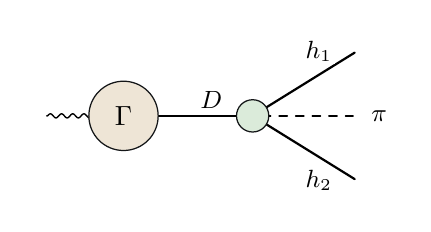
\begin{tikzpicture}[line cap=round, line join=round]
  \begin{feynman}
    \begin{feynhand}
      \vertex (in) at (-1.10,0) {};
      \vertex (src) at (0,0) {};
      \vertex (v) at (1.64,0) {};
      \vertex (top) at (3.06,0.88) {};
      \vertex (mid) at (3.04,0) {};
      \vertex (bot) at (3.06,-0.88) {};
      \path[use as bounding box] (-1.12,-1.12) rectangle (3.55,1.12);

      \propag[pho] (in) to (src);
      \propag[thick] (src) to (v);
      \propag[thick] (v) to (top);
      \propag[sca] (v) to (mid);
      \propag[thick] (v) to (bot);
    \end{feynhand}
  \end{feynman}

  \node[
    draw=pdInk,
    fill=pdSource,
    circle,
    line width=0.45pt,
    minimum size=8.8mm,
    inner sep=0pt
  ] (srcNode) at (src) {$\Gamma$};

  % Feynhand draws incident propagators to (v); the filled vertex masks the
  % unphysical pieces inside the interaction blob.
  \node[
    draw=pdInk,
    fill=pdVertex,
    circle,
    line width=0.45pt,
    minimum size=4.1mm,
    inner sep=0pt
  ] at (v) {};

  \node[pdLabel] at (2.48,0.82) {$h_1$};
  \node[pdLabel] at (2.48,-0.82) {$h_2$};
  \node[pdLabel, right=0.65mm] at (mid) {$\pi$};
  \node[pdLabel, above=0.45mm] at ($(srcNode.east)!0.56!(v)$) {$D$};
\end{tikzpicture}
\end{document}
